\documentclass[german,10pt]{book}      
\usepackage{makeidx}
\usepackage{babel}            % Sprachunterstuetzung
\usepackage{amsmath}          % AMS "Grundpaket"
\usepackage{amssymb,amsfonts,amsthm,amscd} 
\usepackage{mathrsfs}
\usepackage{rotating}
\usepackage{sidecap}
\usepackage{graphicx}
\usepackage{color}
\usepackage{fancybox}
\usepackage{tikz}
\usetikzlibrary{arrows,snakes,backgrounds}
\usepackage{hyperref}
\hypersetup{colorlinks=true,
                    linkcolor=blue,
                    filecolor=magenta,
                    urlcolor=cyan,
                    pdftitle={Overleaf Example},
                    pdfpagemode=FullScreen,}
%\newcommand{\hyperref}[1]{\ref{#1}}
%
\definecolor{Gray}{gray}{0.80}
\DeclareMathSymbol{,}{\mathord}{letters}{"3B}
%
\newcounter{num}
\renewcommand{\thenum}{\arabic{num}}
\newenvironment{anmerkungen}
   {\begin{list}{(\thenum)}{%
   \usecounter{num}%
   \leftmargin0pt
   \itemindent5pt
   \topsep0pt
   \labelwidth0pt}%
   }{\end{list}}
%
\renewcommand{\arraystretch}{1.15}                % in Formeln und Tabellen   
\renewcommand{\baselinestretch}{1.15}                 % 1.15 facher
                                                      % Zeilenabst.
\newcommand{\Anmerkung}[1]{{\begin{footnotesize}#1 \end{footnotesize}}\\[0.2cm]}
\newcommand{\comment}[1]{}
\setlength{\parindent}{0em}           % Nicht einruecken am Anfang der Zeile 

\setlength{\textwidth}{15.4cm}
\setlength{\textheight}{23.0cm}
\setlength{\oddsidemargin}{1.0mm} 
\setlength{\evensidemargin}{-6.5mm}
\setlength{\topmargin}{-10mm} 
\setlength{\headheight}{0mm}
\newcommand{\identity}{{\bf 1}}
%
\newcommand{\vs}{\vspace{0.3cm}}
\newcommand{\noi}{\noindent}
\newcommand{\leer}{}

\newcommand{\engl}[1]{[\textit{#1}]}
\parindent 1.2cm
\sloppy

         \begin{document}  \setcounter{chapter}{0}


\chapter{Physik des Klimas IV\\Treibhausgase}
% Kap x
\label{chap_Klima4}

Als Hauptursache f\"ur den anthropogenen (d.h., vom Menschen erzeugten) Klimawandel
wird heute die Freisetzung von Kohlenstoff in die Atmosph\"are angesehen. Dazu
tragen haupts\"achlich die Verbrennung fossiler Brennstoffe (Kohle, Erdgas) und die
damit verbundene Freisetzung von Kohlendioxid (${\rm CO}_2$) sowie die
Freisetzung von Methan (${\rm CH}_4$) im Zusammenhang mit der Landwirtschaft
(insbesondere der Anbau von Reis sowie gro\ss e Viehherden) bei. 
Andererseits werden Senken von ${\rm CO}_2$, d.h.\ Bereiche, die Kohlendioxid
abbauen und den Kohlenstoff binden, beispielsweise Regenw\"alder, abgebaut bzw.\ 
vernichtet.  

\begin{SCtable}[30][htb]
\begin{tabular}{lr}
Reservoir & Menge \\ \hline
Biosph\"are - Meer & 1 \\
Biosph\"are - Land \& Atmosph\"are & 1 \\
Atmosph\"are (in Form von ${\rm CO}_2$) & 20 \\
Ozean (als gel\"ostes ${\rm CO}_2$) & 4\,000 \\
Fossile Brennstoffe & 800 \\
Ton (shales) &  800\,000 \\
karbonhaltiger Fels (z.B.\ Graphit, Schiefer) & 2\,000\,000 \\ \hline 
\end{tabular}
\caption{\label{tab_GHG1}%
Relative Verteilung von Kohlenstoff in verschiedenen Bereichen nahe der Erdoberfl\"ache.
Die Menge an Kohlenstoff in der heutigen Biomasse an Land bzw.\ im Meer wird willk\"urlich als 1 definiert. 
(Aus \cite{Weyl})
}
\end{SCtable}

Wichtig im Zusammenhang mit dem Klimawandel ist nicht der Kohlenstoff, der sich
im Biozyklus der Erde befindet (in organischen Substanzen), sondern der Kohlenstoff,
der in gebundener Form in Reservoiren vorliegt (z.B.\ in fossilen Brennstoffen; siehe
Tab.\ \ref{tab_GHG1}) und nun
(haupts\"achlich vom Menschen) freigesetzt wird. Dieser Kohlenstoff erh\"oht die Konzentration
in der Luft (in Form von ${\rm CO}_2$ oder ${\rm CH}_4$) oder im Wasser (was z.B.\ zur
Versauerung der Meere f\"uhrt). 
 



\section{Zur fr\"uhen Geschichte der Erforschung der Treibhausgase}

Die Geschichte der Erforschung von Treibhausgasen und ihrem Einfluss auf das Klima
der Erde beginnt mit Joseph Fourier (1768--1830), 
nach dem auch die Fourier-Transformation benannt
ist. Fourier untersuchte die Ausbreitung von W\"arme. In diesem Zusammenhang stie\ss\ er
auf die Diffusionsgleichung und erkannte, dass harmonische Funktionen (Sinus und Kosinus) 
und ihre Linearkombinationen zur L\"osung verwendet werden k\"onnen. In diesem Zusammenhang
stellt er sich die Frage, welche Verteilungsfunktionen sich nach harmonischen Funktionen
entwickeln lassen. Im Jahre 1824 beschrieb er in einem Aufsatz das Grundprinzip des
Treibhauseffekts.

Oft vergessen wird der Beitrag der US-Amerikanerin Eunice Newton Foote (1819--1888). Im Jahre
1856 ver\"offentlichte sie einen Artikel mit dem Titel \textit{Circumstances Affecting the Heat of the
Sun's Rays} im American Journal of Science and Arts \cite{Foote}. 
Darin beschreibt sie die Ergebnisse
ihrer Versuche mit trockener Luft, feuchter Luft und mit Kohlendioxid versetzter Luft, die
sie in einem Glaszylinder dem Sonnenlicht aussetzte. Das Gasgemisch mit erh\"ohtem 
${\rm CO}_2$-Gehalt in der Luft erw\"armte sich am st\"arksten. Sie kommt zu dem Schluss:
\textit{An atmosphere of that gas would give to our earth a high temperature; and if as some
suppose, at one period of its history the air had mixed with it a larger proportion than at
present, an increased temperature from its own action ... must have necessarily resulted.}
Ihr Artikel ist erst im Jahr 2010 im Zusammenhang mit der Untersuchung von Treibhausgasen
entdeckt worden, seither gilt sie als erste Wissenschaftlerin, die
den Zusammenhang zwischen der Konzentration von Kohlendioxid in der Luft und der 
globalen Erw\"armung der Atmosph\"are erkannte.

Der irische Naturforscher John Tyndall (1820--1893) hat 1859 ausf\"uhrliche systematische
Untersuchungen zum Einfluss verschiedener Gase sowie dem Einfluss von infraroter Strahlung
auf die Erw\"armung von Luft durchgef\"uhrt. Er galt bis zur Endeckung der Arbeit von Eunice Foote
als Begr\"under der Theorie des Einflusses von Kohlendioxid auf die globale Erw\"armung
der Erdatmosph\"are. 

Die n\"achsten wichtigen Schritte in der Erforschung von Treibhausgasen auf das Klima
unternahme der schwedische Forscher Svante August Arrhenius (1859--1927). Er
interessierte sich f\"ur die damals allgemein diskutierte Frage, weshalb es \"uberhaupt
Eiszeiten gegeben hat und vermutete einen Zusammenhang zwischen der
CO${}_2$-Konzentration in der Luft und den K\"alteperioden der Eiszeiten. 
Er erstellte sehr ausf\"uhrliche Tabellen zum Einfluss der Konzentration verschiedener 
Gase in Luft auf deren Erw\"armung unter der Einstrahlung infraroter Strahlung.
Zusammen mit seinem Kollegen Arvid Gustaf H\"ogbom (1857--1940) 
stellte er auch als erster die Vermutung auf, dass die Freisetzung von
CO${}_2$ durch die Verbrennung fossiler Brennstoffe
zu einer anthropogenen globalen Erw\"armung des Klimas f\"uhren k\"onnte. 

\section{Die Keeling-Kurve}

Mitte der 50er Jahre des letzten Jahrhunderts untersuchte der amerikanische Chemiker
Charles David Keeling (1928--2005) den ${\rm CO}_2$-Gehalt der Luft an der Westk\"uste
Amerikas und stellte tageszeitliche Schwankungen fest. Um genauere und vom Stra\ss enverkehr 
und industriellen Einfl\"ussen unabh\"angige Daten zu erhalten, ging er 1957 nach Hawaii
und begann dort mit Messungen des Kohlendioxidgehalts der Luft auf dem Mauna Loa, dem
zweith\"ochsten Vulkan auf der Hauptinsel von Hawaii. Seit 1958 werden von einem
Observatorium auf dem Mauna Loa st\"undlich ${\rm CO}_2$-Messungen durchgef\"uhrt (siehe
Abb.\ \ref{fig_Keeling1}). 

\begin{figure}[htb]
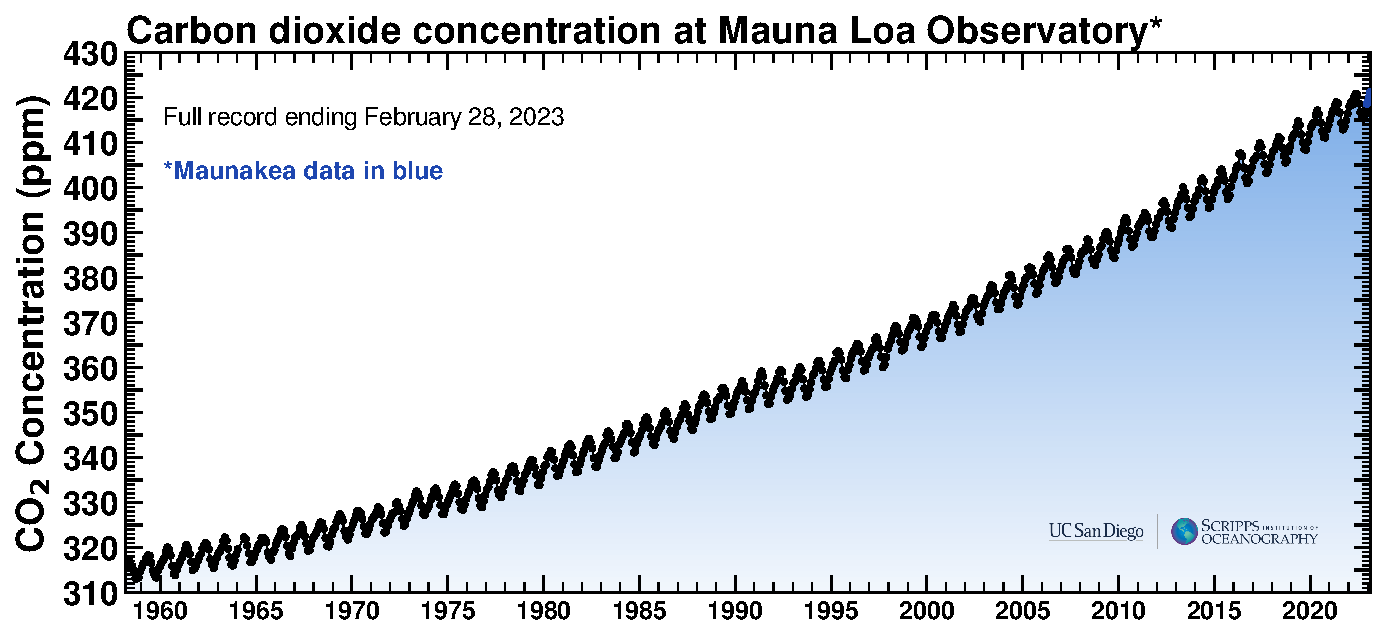
\includegraphics[scale=0.6]{./Bilder/full_record.pdf}
\caption{\label{fig_Keeling1}%
Die Keeling-Kurve. Dargestellt sind die Ergebnisse von ${\rm CO}_2$-Messungen
am Mauna Loa, Hawaii (monatliche Mittelwerte). W\"ahrend der Zeit zwischen
November 2022 und M\"arz 2023 wurden die Messungen wegen eines
Vulkanausbruchs am Mauna Loa auf dem benachbarten Maunakea 
durchgef\"uhrt. (von \cite{Keeling})}
\end{figure}

Die Kohlendioxidkonzentrationen sind in ppm (parts per million) angegeben. Im Mai 2022 wurde
zum ersten Mal die 420\,ppm Marke \"uberschritten. Begonnen hat die Kurve 1958 bei
Werten von rund 315\,ppm. Die Kurve zeigt deutliche jahreszeitliche Schwankungen: In den
Monaten Mai bis September nimmt die Konzentration ab, in den Monaten
von Oktober bis April nimmt die Konzentration wieder zu. Dieses Verhalten wird mit der
vermehrten Aufnahme von Kohlendioxid durch die Pflanzenwelt auf der n\"ordlichen
Halbkugel in den Fr\"uhjahrs- und Sommermonaten erkl\"art. Die Nordhalbkugel hat
deutlich mehr bepflanzte Landfl\"achen als die S\"udhalbkugel, sodass haupts\"achlich
dieser Einfluss sichtbar wird. 

Erstaunlich ist auch, dass beispielsweise w\"ahrend der
Corona-Pandemie, wo der Flugverkehr sowie der Autoverkehr deutlich geringer waren, kaum
ein Effekt auf die CO${}_2$-Konzentration der Atmosph\"are sichtbar ist. Auch die
angeblich intensiven Bem\"uhungen der Staatengemeinschaft, den CO${}_2$-Aussto\ss\ 
deutlich zu reduzieren, machen sich bisher kaum bemerkbar. Allerdings zeigen die Daten
hier, dass in der weltweiten Summe die CO${}_2$-Emissionen weiterhin zunehmen, im Wesentlichen
durch die Zuw\"achse in China und Indien (siehe Abb.\ \ref{fig_co2}). In den Vereinigten
Staaten haben die CO${}_2$-Emissionen erst um 2007 abgenommen und die USA liegen immer
noch nach China an der zweiten Stelle in Bezug auf die absoluten Emissionswerte.
Andererseits hat Deutschland einen \"ahnlichen pro Kopf 
Verbrauch wie China. Nach einigen
arabische Staaten sowie Kanada und Australien sind die USA hier f\"uhrend (\cite{ProKopf}).  


\begin{figure}[htb]
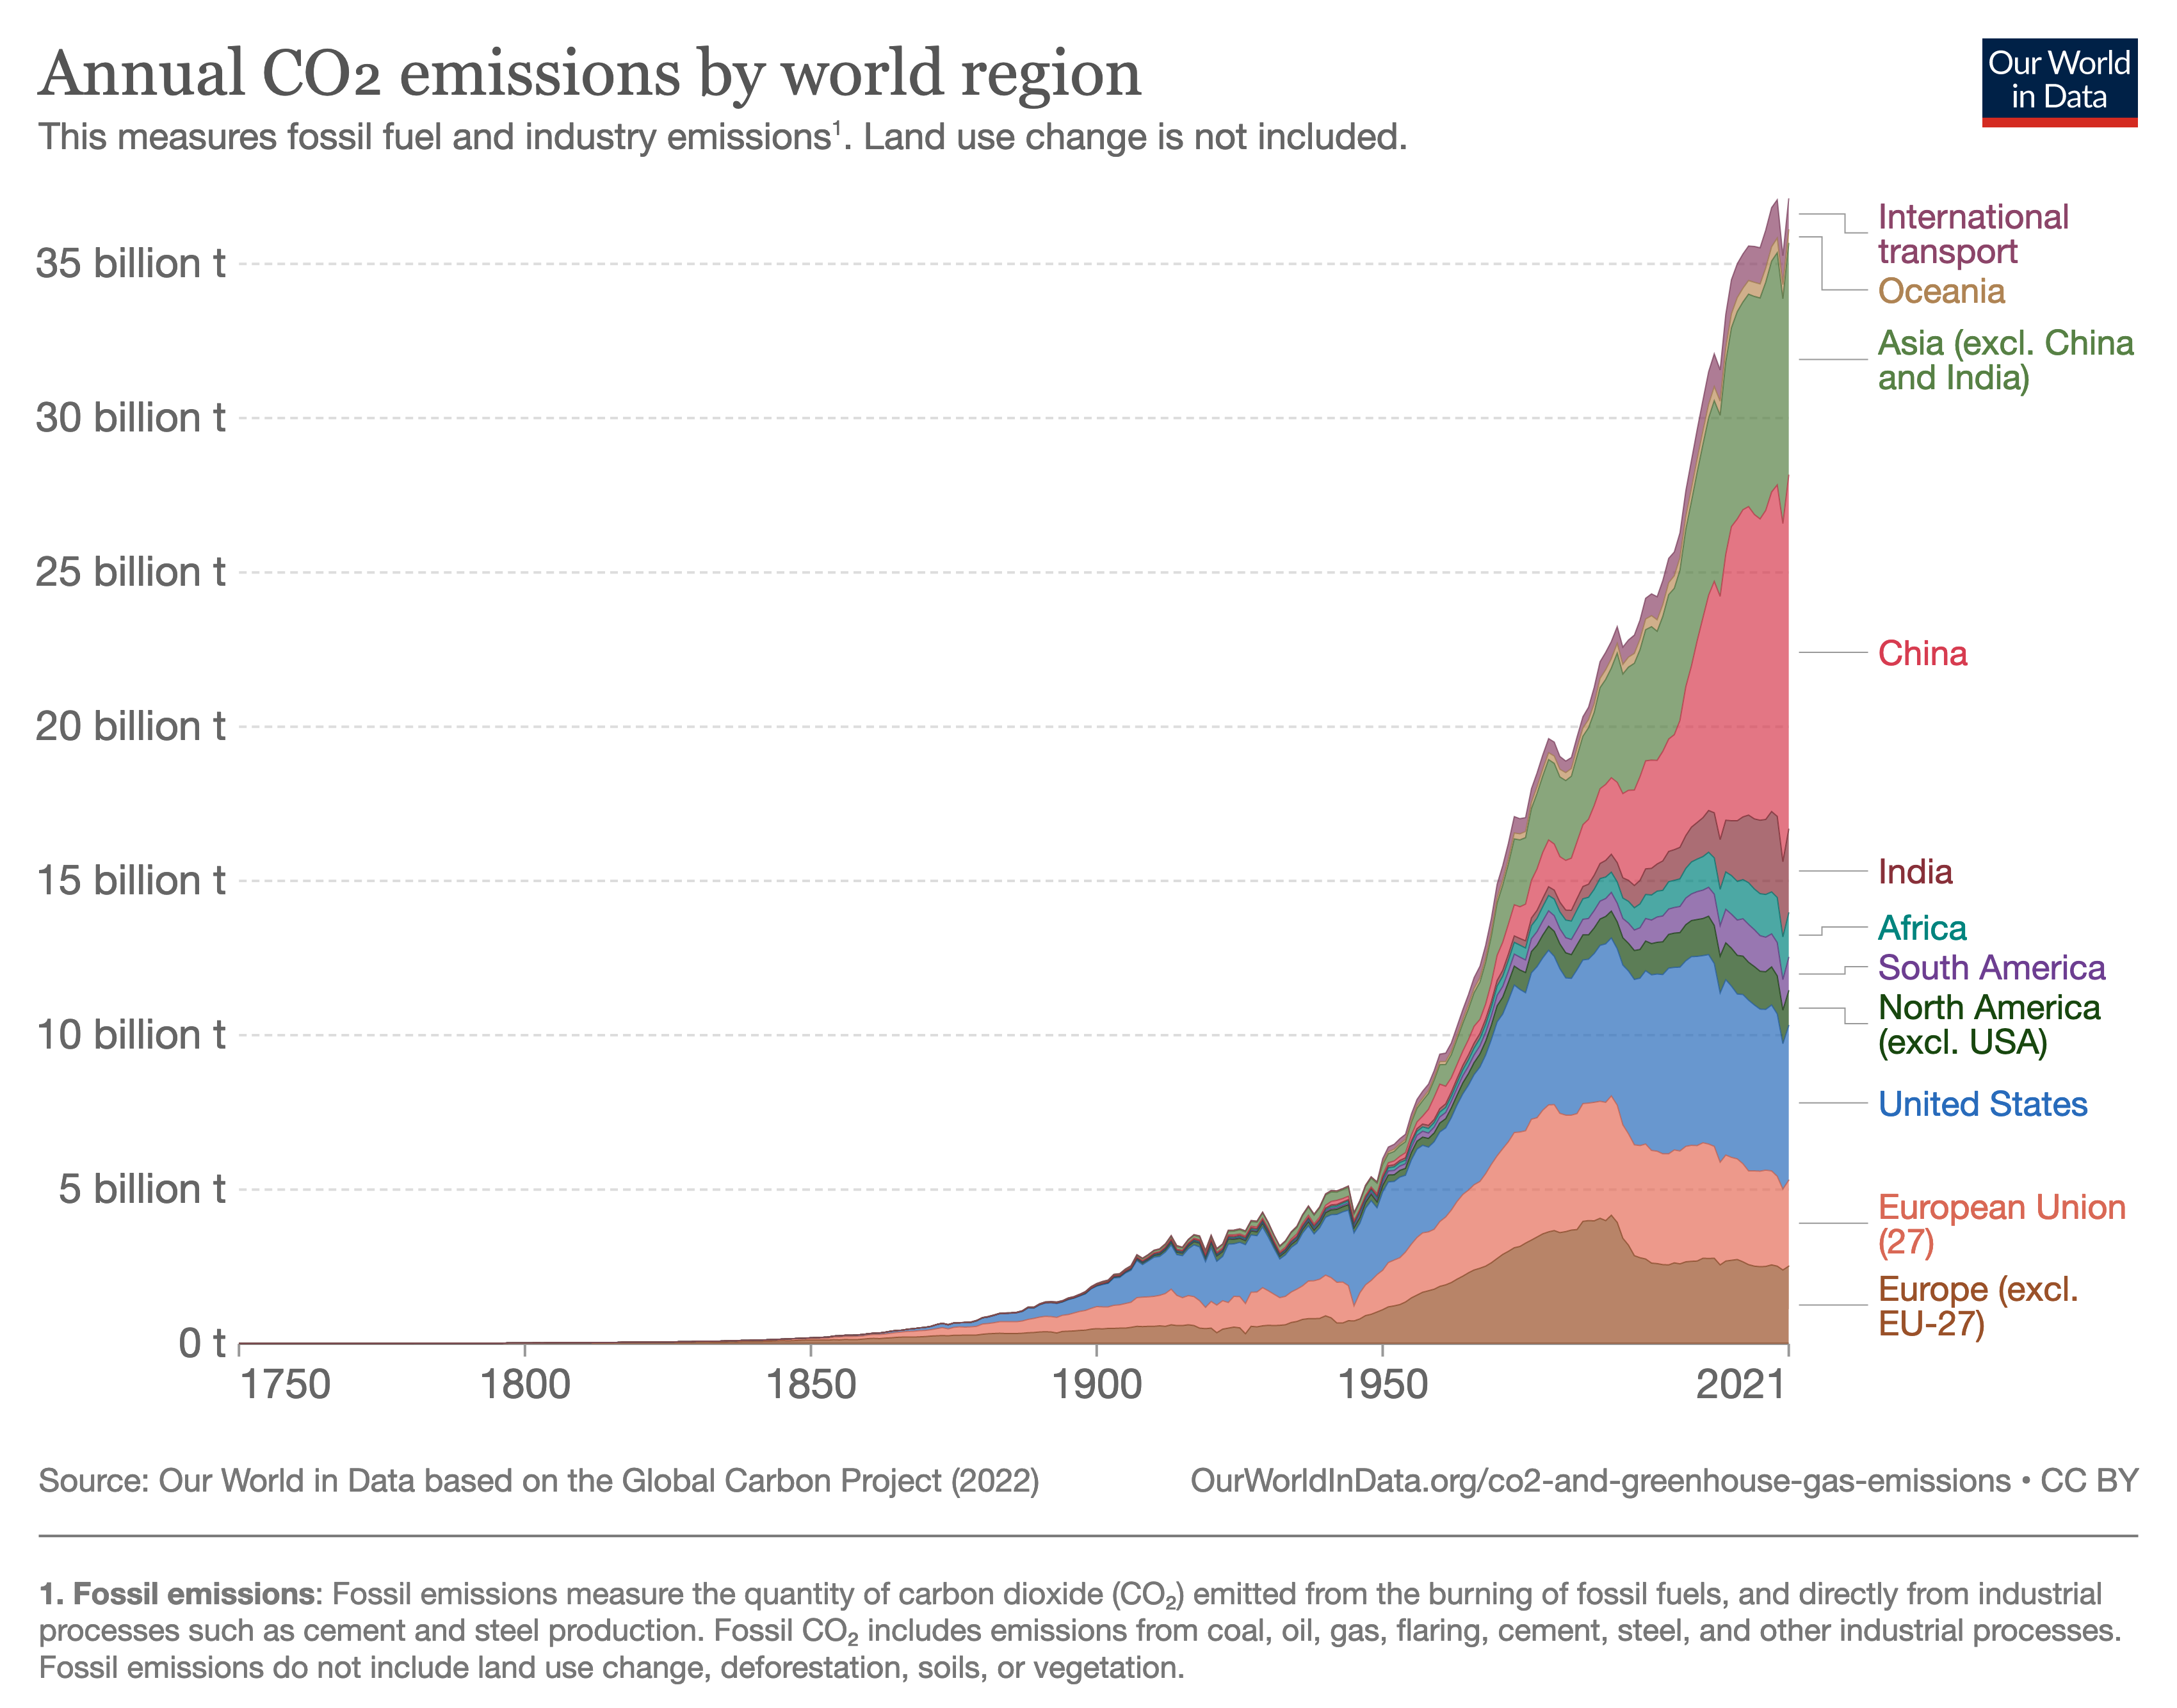
\includegraphics[scale=0.064]{./Bilder/annual-co-emissions-by-region.png}
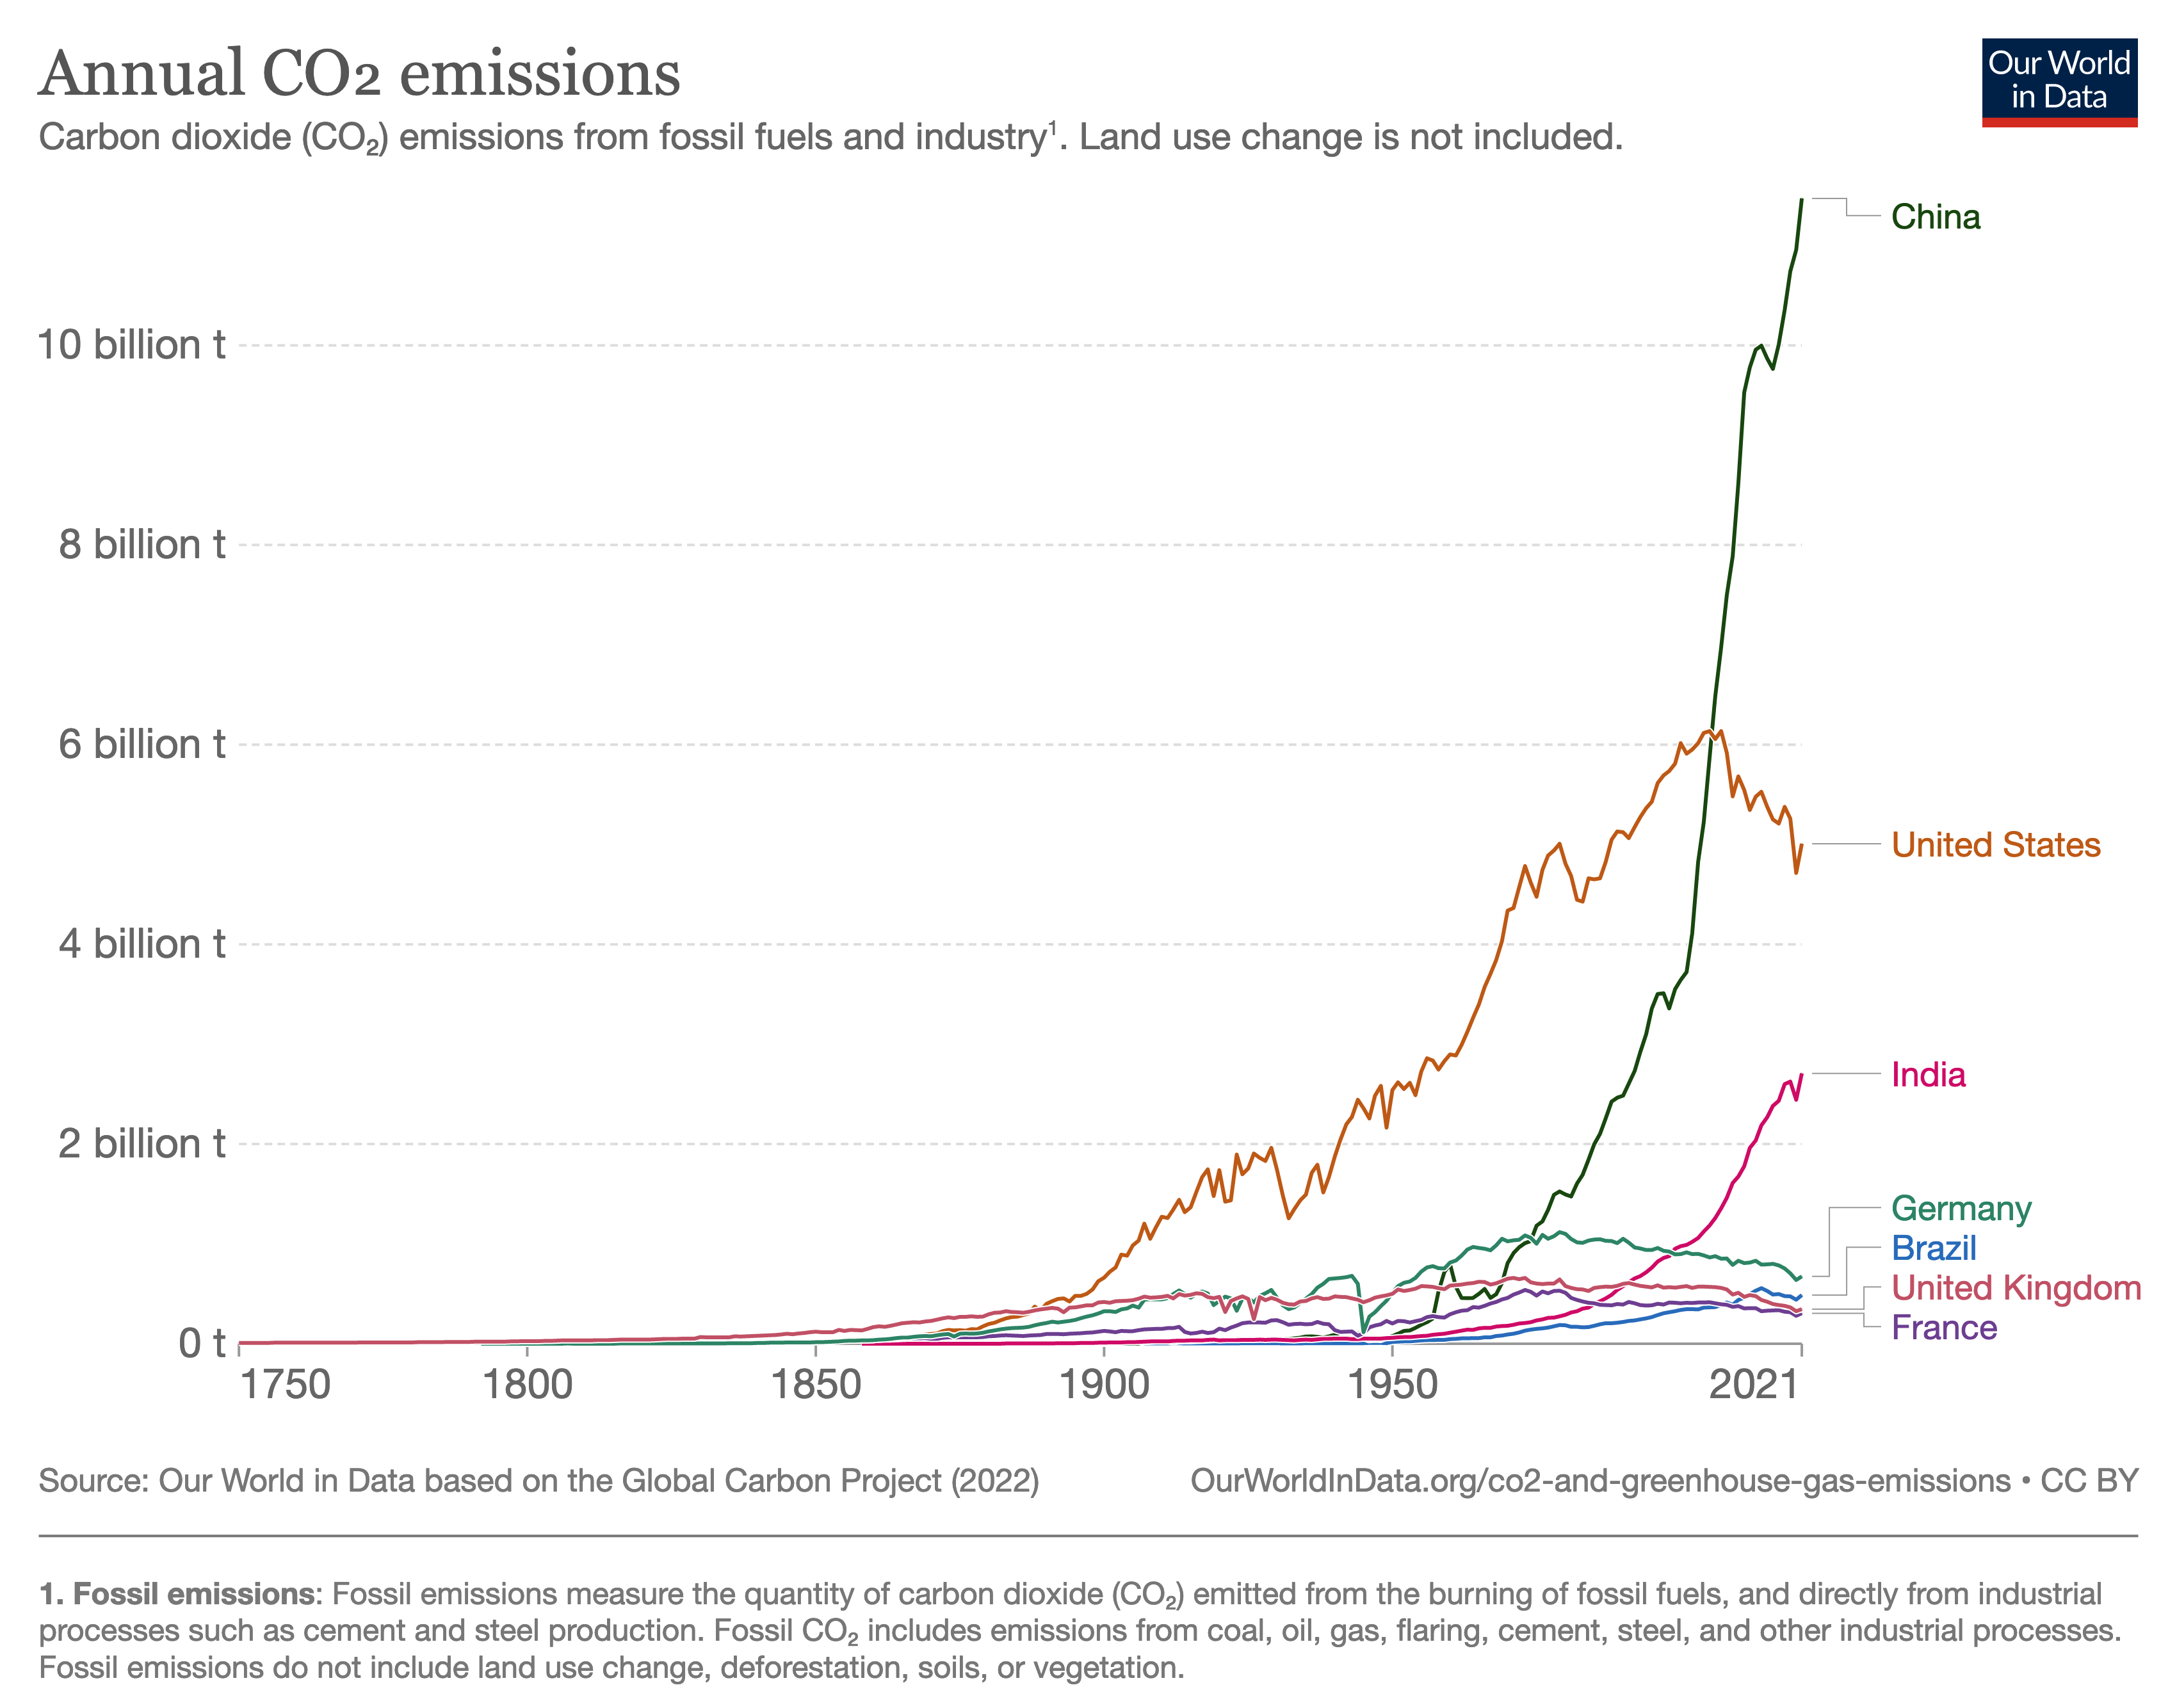
\includegraphics[scale=0.064]{./Bilder/annual-co2-emissions-per-country.png}
\caption{\label{fig_co2}%
CO${}_2$-Emissionen nach Gebieten, kumulativ (links), sowie nach L\"andern (rechts). 
(Aus \cite{WorldData})}
\end{figure}

Man kann den CO${}_2$-Gehalt der Atmosph\"are auch historisch weiter zur\"uckverfolgen.
Dazu verwendet man die Daten von Eisborungen in der Antarktis und der Arktis. Im Eis sind
winzige Luftbl\"aschen gefangen, deren CO${}_2$-Gehalt bestimmt werden kann. Diese
Daten schlie\ss en sich nahtlos an die Keeling-Kurve an und stimmen in den neueren
Jahren mit ihr \"uberein. Betrachtet man hier die letzten 10\,000 Jahre, so erkennt man,
dass der CO${}_2$-Gehalte der Atmosph\"are bis rund 1750 nahezu konstant geblieben ist
und ab Ende des 18.\ Jahrhunderts (dem Beginn der industriellen Revolution) deutlich
ansteigt (siehe Abb.\ \ref{fig_Keeling2}, links). Man bezeichnet diese Kurve wegen ihres nahezu 
geraden Verlaufs bis zum Ende des 18.\ Jahrhunderts und ihrem anschlie\ss enden steilen Anstieg
auch oft als \glqq Hockeyschl\"ager-Kurve\grqq.
 
\begin{figure}[htb]
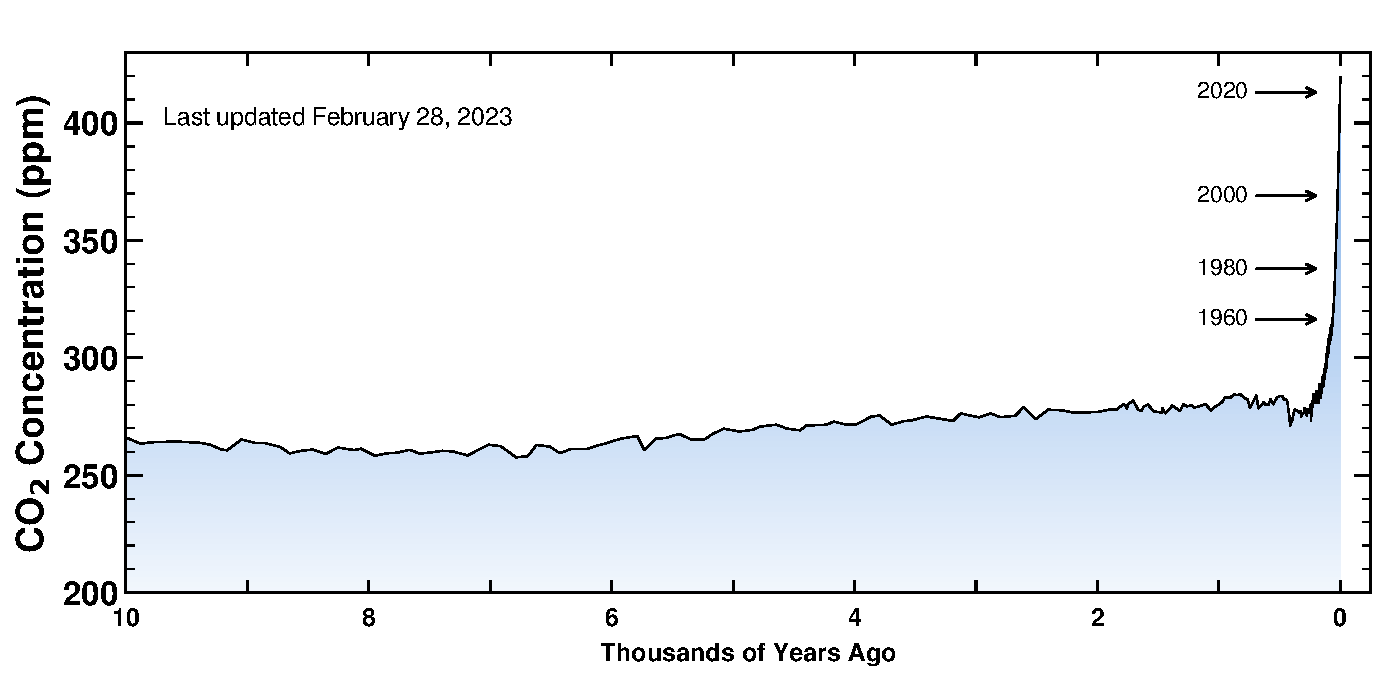
\includegraphics[scale=0.32]{./Bilder/co2_10k.pdf}
\hfill
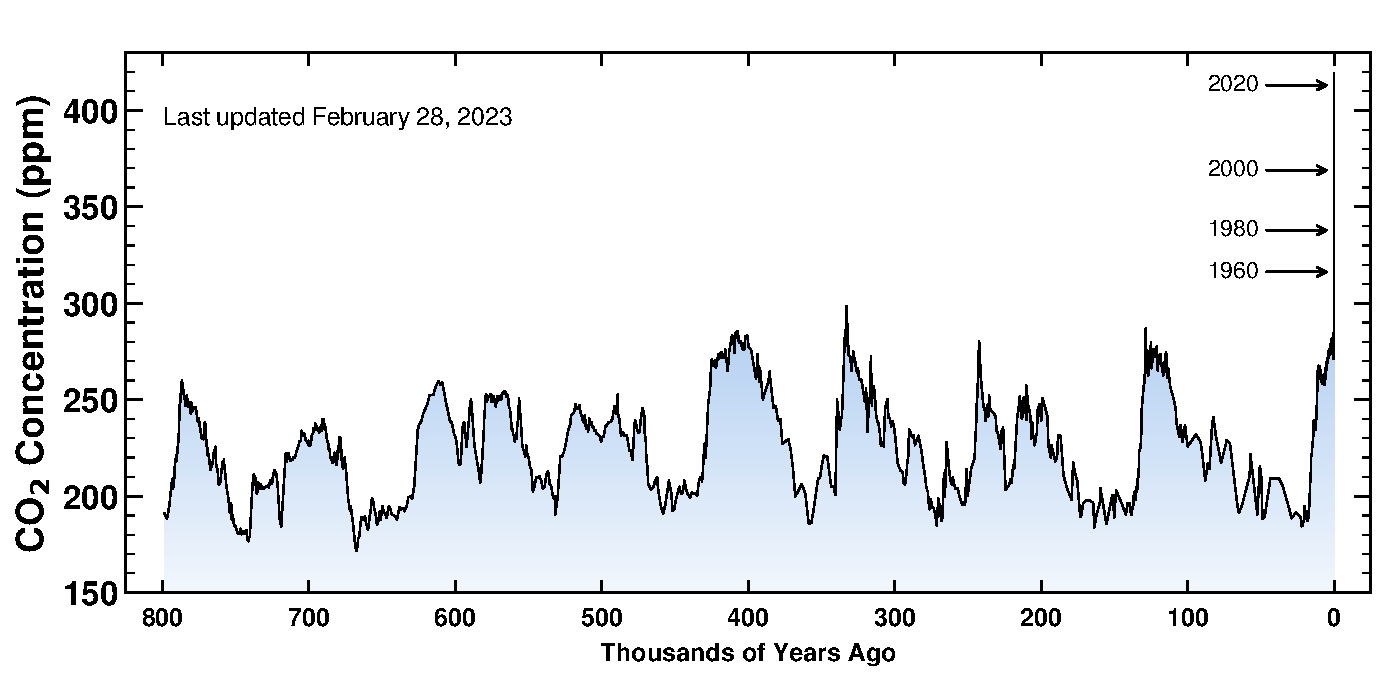
\includegraphics[scale=0.32]{./Bilder/co2_800k.pdf}
\caption{\label{fig_Keeling2}%
(links) CO${}_2$-Gehalt der Atmosph\"are in den letzten 10\,000 Jahren, (rechts) in den
letzten 800\,000 Jahren. (Aus \cite{Keeling})}  
\end{figure} 

Die Daten der letzten 800\,000 Jahre (siehe Abb.\ \ref{fig_Keeling2}, rechts) zeigen, dass
es immer wieder Schwankungen zwischen rund 170\,ppm und 300\,ppm gab. Diese
Schwankungen korrelieren deutlich mit den Eiszeiten (wenn der CO${}_2$-Gehalt der
Atmosph\"are niedrig war) bzw.\ den Zwischeneiszeiten (mit hohem CO${}_2$-Gehalt). 
Diese Diagramme zeigen, dass wir derzeit in einer vergleichsweise warmen Periode
der letzten 800\,000 Jahre leben. Allerdings gab es in fr\"uheren Zeiten (z.B.\ der
Kreidezeit) noch deutlich w\"armere Perioden (siehe Kap.\ \ref{chap_klima1}). 

\section{Treibhausgase und ihre Absorbtionsspektren}

Das bei weitem wichtigste Treibhausgas ist Wasserdampf. Da die haupts\"achlichen Bestandteile 
der Luft - Stickstoff, Sauerstoff und
Argon - keine Treibhausgase sind, ist Wasserdampf trotz seiner geringen Konzentration von
0--4\% (je nach Luftfeuchtigkeit) das h\"aufigste Treibhausgas in unserer Atmosph\"are.
Es erf\"ullt eine doppelte Aufgabe im Zusammenhang mit der Oberfl\"achentemperatur der
Erde: Zum einen sorgen Wolken, also kondensiertes Wasser, f\"ur den Hauptbeitrag zur
Albedo der Erde, und zum anderen absorbiert Wasserdampf einen gro\ss en Anteil 
der von der Erdoberfl\"ache emittierten Strahlung im Infrarotbereich (IR)
und tr\"agt so zum Treibhauseffekt der Erdoberfl\"ache bei.  



\section{Anmerkungen}

\begin{anmerkungen}
\item
\label{Anm-1}%
Der Grund f\"ur den Faktor 2 zwischen der Schwankung im Abstand und
der Schwankung in der Intensit\"at der Sonneneinstrahlung liegt in dem $1/r^2$-Gesetz
der Intensit\"at als Funktion des Abstands:
\begin{equation}
        \frac{1}{(r\pm \Delta r)^2} \approx \frac{1}{r^2} \mp 2 \frac{\Delta r}{r} \, .
\end{equation}

\end{anmerkungen}



\begin{thebibliography}{99}
\bibitem{AR6} IPCC Assessment Report 6 ???,\\
       {\small \verb+https://www.ipcc.ch/assessment-report/ar6/+}   
\bibitem{Foote} Eunice Newton Foote; \textit{Circumstances affecting the Heat  of the Sun's Rays};
          American Journal of Science and Arts, 1856; p.\ 382--383. abrufbar unter Wikipedia
          \glqq Eunice Newton Foote\grqq, \url{https://en.wikipedia.org/wiki/Eunice_Newton_Foote}
          (abgerufen am 13.4.2023).         
\bibitem{Keeling} Keeling-Kurve, Scripps CO2-program, Scripps Institution of Oceanography, San Diego;\\
           \url{https://keelingcurve.ucsd.edu/}        
\bibitem{WorldData} Webseite: \glqq Our World in Data\grqq,         
           \url{https://ourworldindata.org/co2-emissions}        
\bibitem{ProKopf} aus Wikipedia \glqq List of countries by carbon dioxide emissions per capita\grqq.
\bibitem{Weyl} P.\,K.\,Weyl; \textit{Oceanography}; John Wiley \& Sons, New York, 1970.\\
    aus \url{https://www.youtube.com/watch?v=MTLInONp-Z4&t=87s}; 1:18--2:33.
\end{thebibliography}

\end{document}

